\section{Jensen's formula and the variance profile}\label{sec:radial}

By Jensen's formula, the number of roots in a disk is the slope of the
angular logarithm $J_N(e^t)$, a convex function of $t$, so bounds on
$J_N$ at four radii bound the roots outside an annulus. Replacing $J_N$
by its Gaussian value, which Proposition~\ref{prop:profiles} computes,
gives the limiting fraction. Let $f_N(z)=\sum_{k=0}^N\epsilon_kz^k$, and
set
\[
 \sigma_N(r)^2=\sum_{k=0}^Nr^{2k},\qquad
 J_N(r)=\int_{\mathbb T}\log|f_N(re^{i\theta})|\dd\mu(\theta).
\]
The results of this section hold for every nonzero polynomial $f_N$ of
degree at most $N$; randomness enters only through
Section~\ref{sec:concentration}. We write $\gamma$ for Euler's constant.

\begin{lemma}[Four-radius bound for radial mass]\label{thm:T2}
Let $f_N$ be a nonzero polynomial of degree at most $N$, and fix $K>0$,
$0<\eta<1$ and $N>K$. We set
\[
 (x_1,x_2,x_3,x_4)=(-K,-(1-\eta)K,(1-\eta)K,K),\qquad r_i=1+x_i/N.
\]
Let $\sigma_N(r)>0$ be a normalization, and suppose that at each of these
four radii
\begin{equation}
 \left|J_N(r_i)-\log\sigma_N(r_i)+\gamma/2\right|\leq\varepsilon_i,
 \qquad i=1,2,3,4. \label{eq:four-radius-log-errors}
\end{equation}
Then
\begin{align}
 \frac{\#\{\alpha:f_N(\alpha)=0,\ ||\alpha|-1|>K/N\}}N
 &\leq\frac{\deg f_N}N\nonumber\\
 &\quad+\frac{\log\sigma_N(r_2)-\log\sigma_N(r_1)+\varepsilon_1+\varepsilon_2}{N\log(r_2/r_1)}\nonumber\\
 &\quad-\frac{\log\sigma_N(r_4)-\log\sigma_N(r_3)-\varepsilon_3-\varepsilon_4}{N\log(r_4/r_3)}.\label{eq:T2-exact}
\end{align}
In particular, suppose that along a sequence of degrees $\deg f_N/N\to1$, that
the errors $\varepsilon_i$ tend to zero, and that $\log\sigma_N(1+x/N)$,
minus a deterministic centering that may depend on $N$ but not on $x$,
converges to $F(x)$ uniformly on $[-K,K]$.
Then the limiting upper bound for
$\#\{\alpha:f_N(\alpha)=0,\ ||\alpha|-1|>K/N\}/N$ is
\begin{equation}
 1+\frac1{\eta K}\{F(-(1-\eta)K)-F(-K)-F(K)+F((1-\eta)K)\}. \label{eq:T2-limit}
\end{equation}
\end{lemma}

We call $r_1,\dots,r_4$ the secant radii. Here the centering $-\gamma/2$ is $\E\log|G|$, where $G$ has density
$\pi^{-1}e^{-|z|^2}$ on $\C$, and it is the same at all four radii.
If the four bounds \eqref{eq:four-radius-log-errors} hold outside four
exceptional events, then \eqref{eq:T2-exact} holds outside their union,
whose probability is at most the sum of their probabilities.
The limiting bound \eqref{eq:T2-limit} holds for every sample sequence on
which the four bounds hold for all sufficiently large degrees.

\begin{proof}
We bound the roots in $\{|z|<r_1\}$ and in $\{|z|>r_4\}$ by the slopes
of two secants of the convex function $t\mapsto J_N(e^t)$, and then
replace $J_N$ by $\log\sigma_N$ using \eqref{eq:four-radius-log-errors}.
Write $f_N(z)=a\prod_{j=1}^{\deg f_N}(z-\alpha_j)$.
By Jensen's formula \cite[\S3.61]{Titchmarsh1939} for one factor,
$\int_{\mathbb T}\log|e^te^{i\theta}-\alpha|\dd\mu(\theta)=\max(t,\log|\alpha|)$
for $\alpha\ne0$, and the integral is $t$ for $\alpha=0$, so that
\[
 J_N(e^t)=\log|a|+\sum_{j=1}^{\deg f_N}\max(t,\log|\alpha_j|),
 \qquad t\in\mathbb R,
\]
where a term with $\alpha_j=0$ is read as $t$. The term of $\alpha_j$ has
right derivative $1$ if $|\alpha_j|\le e^t$ and $0$ otherwise, so
$t\mapsto J_N(e^t)$ is convex and piecewise linear with right derivative
$\nu_N(e^t)$. Integrating it and substituting $r=e^s$, we get
\begin{equation}
 J_N(e^{t'})-J_N(e^t)=\int_t^{t'}\nu_N(e^s)\dd s
 =\int_{e^t}^{e^{t'}}\frac{\nu_N(r)}r\dd r,\qquad t<t'.
 \label{eq:jensen-integral}
\end{equation}

Since $N>K$, we have $0<r_1<r_2<r_3<r_4$, and since $\nu_N$ is
nondecreasing, \eqref{eq:jensen-integral} gives
\begin{align*}
 \nu_N(r_1)
 &\leq\frac1{\log(r_2/r_1)}\int_{r_1}^{r_2}\frac{\nu_N(r)}r\dd r
 =\frac{J_N(r_2)-J_N(r_1)}{\log(r_2/r_1)},\\
 \frac{J_N(r_4)-J_N(r_3)}{\log(r_4/r_3)}
 &=\frac1{\log(r_4/r_3)}\int_{r_3}^{r_4}\frac{\nu_N(r)}r\dd r
 \leq\nu_N(r_4).
\end{align*}
By \eqref{eq:four-radius-log-errors}, in which $\gamma/2$ cancels in
differences, we have
\begin{align*}
 J_N(r_2)-J_N(r_1)
 &\leq\log\sigma_N(r_2)-\log\sigma_N(r_1)+\varepsilon_1+\varepsilon_2,\\
 J_N(r_4)-J_N(r_3)
 &\geq\log\sigma_N(r_4)-\log\sigma_N(r_3)-\varepsilon_3-\varepsilon_4.
\end{align*}

Let $m$ be the number of roots with $||\alpha|-1|>K/N$. At most
$\nu_N(r_1)$ of them lie in $\{|z|<r_1\}$ and exactly
$\deg f_N-\nu_N(r_4)$ in $\{|z|>r_4\}$, so by the last two displays
\begin{align*}
 \frac mN
 &\leq\frac{\nu_N(r_1)}N+\frac{\deg f_N-\nu_N(r_4)}N
 \leq\frac{\deg f_N}N
   +\frac{J_N(r_2)-J_N(r_1)}{N\log(r_2/r_1)}
   -\frac{J_N(r_4)-J_N(r_3)}{N\log(r_4/r_3)}\\
 &\leq\frac{\deg f_N}N
   +\frac{\log\sigma_N(r_2)-\log\sigma_N(r_1)+\varepsilon_1+\varepsilon_2}{N\log(r_2/r_1)}\\
 &\quad-\frac{\log\sigma_N(r_4)-\log\sigma_N(r_3)-\varepsilon_3-\varepsilon_4}{N\log(r_4/r_3)}.
\end{align*}
This proves \eqref{eq:T2-exact}.

For the limit, let $c$ be the centering of the hypothesis and
$F_N(x)=\log\sigma_N(1+x/N)-c$, so that $\log\sigma_N(r_i)=F_N(x_i)+c$.
Then
\begin{align*}
 N\log(r_2/r_1)&=\int_{-K}^{-(1-\eta)K}\frac{\mathrm dx}{1+x/N}\longrightarrow\eta K,\\
 N\log(r_4/r_3)&=\int_{(1-\eta)K}^{K}\frac{\mathrm dx}{1+x/N}\longrightarrow\eta K.
\end{align*}
Since $c$ cancels in differences, the right-hand side of
\eqref{eq:T2-exact} is the first line below, and since $\deg f_N/N\to1$,
$\varepsilon_i\to0$ and $F_N(x_i)\to F(x_i)$,
\begin{align*}
 &\frac{\deg f_N}N
   +\frac{F_N(x_2)-F_N(x_1)+\varepsilon_1+\varepsilon_2}{N\log(r_2/r_1)}
 -\frac{F_N(x_4)-F_N(x_3)-\varepsilon_3-\varepsilon_4}{N\log(r_4/r_3)}\\
 &\qquad\longrightarrow1+\frac{F(x_2)-F(x_1)}{\eta K}-\frac{F(x_4)-F(x_3)}{\eta K},
\end{align*}
so that the limit superior of $m/N$ is at most \eqref{eq:T2-limit}.
\end{proof}

Figure~\ref{fig:jensen-secants} shows these secants for one sequence at $N=10^5$.
Section~\ref{sec:log-rate} lets $\eta$ tend to zero with $N$, and all
other uses take $\eta=1/2$.

\begin{figure}[t]
\centering
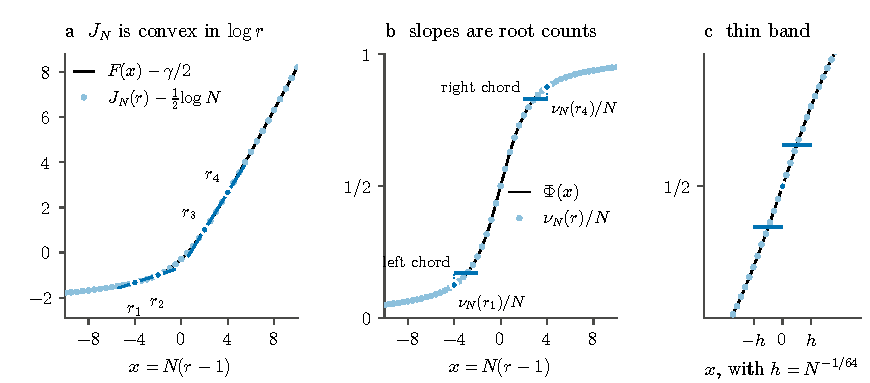
\includegraphics[width=\textwidth]{figures/explanatory/jensen-secants.pdf}
\caption{Jensen secants for one sequence at $N=10^5$. The chord slopes bound
the normalized zero counts, which approach $\Phi$.}
\label{fig:jensen-secants}
\end{figure}


\begin{proposition}[The unweighted logarithmic variance profile]\label{prop:profiles}
For the normalization $\sigma_N(r)^2=\sum_{k=0}^Nr^{2k}$ of this section,
\[
 \log\sigma_N(1+x/N)-\tfrac12\log N\longrightarrow
 F(x):=\frac12\log\int_0^1e^{2xt}\dd t
\]
uniformly on compact intervals of $x$. The profile satisfies
\[
 F'(x)=\Phi(x),\qquad F(x)=x+F(-x),\qquad F'(0)=\tfrac12.
\]
For $0<\eta<1$, the bound in \eqref{eq:T2-limit} is
\begin{equation}
 \frac2{\eta K}\{F(-(1-\eta)K)-F(-K)\}
 =\frac1{\eta K}\log\frac{1-e^{-2(1-\eta)K}}{(1-\eta)(1-e^{-2K})}
 \le\frac1{\eta K}\log\frac1{1-\eta},
 \label{eq:profile-eta-bound}
\end{equation}
which at $\eta=1/2$ is
\[
 \frac2K\log\frac{2}{1+e^{-K}}\leq\frac{2\log2}{K}.
\]
\end{proposition}

\begin{proof}
We first compare each term $(1+x/N)^{2k}$ of $\sigma_N(1+x/N)^2$ with
$e^{2xk/N}$, which turns $\sigma_N(1+x/N)^2/N$ into a Riemann sum for
$\int_0^1e^{2xt}\dd t$, and then derive the identities for $F$ and the
value of \eqref{eq:T2-limit} from this integral.

For $|x|\leq K$, $N\geq2K$ and $0\leq k\leq N$, expanding the logarithm
in its power series and using $|x/N|\le K/N\le1/2$, we obtain
\begin{align*}
 &\left|2k\log(1+x/N)-2xk/N\right|
 =2k\left|-\frac12\Big(\frac xN\Big)^2+\frac13\Big(\frac xN\Big)^3-\cdots\right|\\
 &\qquad\le k\Big(\frac xN\Big)^2\Big(1+\Big|\frac xN\Big|+\Big(\frac xN\Big)^2+\cdots\Big)
 =\frac{k(x/N)^2}{1-|x/N|}\le2k\Big(\frac xN\Big)^2\le2K^2/N.
\end{align*}
Exponentiating, we get
\begin{equation}
 e^{-2K^2/N}\leq
 \frac{(1+x/N)^{2k}}{e^{2xk/N}}\leq e^{2K^2/N}.
 \label{eq:profile-comparison}
\end{equation}

Since $(x,t)\mapsto e^{2xt}$ is uniformly continuous on
$[-K,K]\times[0,1]$ and the term $k=0$ is $1/N$, the Riemann sums
$\frac1N\sum_{k=0}^Ne^{2xk/N}$ converge to $\int_0^1e^{2xt}\dd t$
uniformly for $|x|\leq K$. Multiplying \eqref{eq:profile-comparison} by
$e^{2xk/N}/N$ and summing over $0\le k\le N$, we see that
$\sigma_N(1+x/N)^2/N=\frac1N\sum_{k=0}^N(1+x/N)^{2k}$ lies between
$e^{-2K^2/N}$ and $e^{2K^2/N}$ times the Riemann sum, so that it has the
same limit. Since this limit is at least $e^{-2K}$ and the logarithm is
uniformly continuous on $[e^{-2K}/2,\infty)$, we obtain, uniformly for
$|x|\le K$,
\[
 \log\sigma_N(1+x/N)-\tfrac12\log N
 =\frac12\log\frac{\sigma_N(1+x/N)^2}N
 \longrightarrow\frac12\log\int_0^1e^{2xt}\dd t
 =F(x).
\]

Differentiating the positive integral under the integral sign, we have
\[
 F'(x)=\frac12\,\frac{\int_0^12te^{2xt}\dd t}{\int_0^1e^{2xt}\dd t}
 =\frac{\int_0^1t e^{2xt}\dd t}{\int_0^1e^{2xt}\dd t}
 =\Phi(x),
\]
and in particular $F'(0)=\int_0^1t\dd t=\frac12$.
Thus $\Phi(x)$ is the mean of $t$ under the probability density
proportional to $e^{2xt}$ on $[0,1]$, so that $0\le\Phi\le1$, and
differentiating this mean under the integral sign we get
\begin{align}
 \Phi'(x)
 &=\frac{\mathrm d}{\mathrm dx}\,\frac{\int_0^1te^{2xt}\dd t}{\int_0^1e^{2xt}\dd t}
 =\frac{\int_0^12t^2e^{2xt}\dd t}{\int_0^1e^{2xt}\dd t}
  -\frac{\int_0^1te^{2xt}\dd t\int_0^12te^{2xt}\dd t}{\bigl(\int_0^1e^{2xt}\dd t\bigr)^2}\nonumber\\
 &=2\bigg(\frac{\int_0^1t^2e^{2xt}\dd t}{\int_0^1e^{2xt}\dd t}
  -\Big(\frac{\int_0^1te^{2xt}\dd t}{\int_0^1e^{2xt}\dd t}\Big)^2\bigg)
 =2\operatorname{Var}_x(t)\ge0,\label{eq:Phi-variance}
\end{align}
where $\operatorname{Var}_x(t)$ is the variance of $t$ under the same
density.
The change of variables $t\mapsto1-t$ gives the symmetry
\[
 F(x)=\frac12\log\int_0^1e^{2x(1-t)}\dd t
 =\frac12\log\Big(e^{2x}\int_0^1e^{-2xt}\dd t\Big)
 =x+F(-x).
\]
By integration we also obtain, for $y>0$, $\int_0^1e^{-2yt}\dd t=(1-e^{-2y})/(2y)$, and hence
\begin{align*}
 F(-(1-\eta)K)-F(-K)
 &=\frac12\log\frac{(1-e^{-2(1-\eta)K})/(2(1-\eta)K)}{(1-e^{-2K})/(2K)}\\
 &=\frac12\log\frac{1-e^{-2(1-\eta)K}}{(1-\eta)(1-e^{-2K})}
 \le\frac12\log\frac1{1-\eta},
\end{align*}
since $1-e^{-2(1-\eta)K}\le1-e^{-2K}$. At $\eta=1/2$ the expression
before the inequality is
\[
 F(-K/2)-F(-K)=\frac12\log\frac{2(1-e^{-K})}{1-e^{-2K}}
 =\frac12\log\frac2{1+e^{-K}}.
\]
By $F(x)=x+F(-x)$ at $x=K$ and at $x=(1-\eta)K$,
\begin{align*}
 F(K)-F((1-\eta)K)&=K+F(-K)-(1-\eta)K-F(-(1-\eta)K)\\
 &=\eta K+F(-K)-F(-(1-\eta)K),
\end{align*}
and substituting this into \eqref{eq:T2-limit} we get
\begin{align*}
 &1+\frac1{\eta K}\{F(-(1-\eta)K)-F(-K)-F(K)+F((1-\eta)K)\}\\
 &\qquad=1+\frac1{\eta K}\{2F(-(1-\eta)K)-2F(-K)-\eta K\}\\
 &\qquad=\frac2{\eta K}\{F(-(1-\eta)K)-F(-K)\},
\end{align*}
which is \eqref{eq:profile-eta-bound} by the evaluation of
$F(-(1-\eta)K)-F(-K)$ above, and at $\eta=1/2$ is
\[
 \frac2K\log\frac2{1+e^{-K}}\le\frac{2\log2}K.
\]
\end{proof}

This proof also yields a rate of convergence in the profile limit.

\begin{lemma}[Rate in the variance profile]\label{lem:profile-rate}
For $K>0$, $N\ge2K$ and $|x|\le K$,
\[
 \left|\log\sigma_N(1+x/N)-\tfrac12\log N-F(x)\right|
 \le\frac{K^2+e^{4K}/2}{N}.
\]
\end{lemma}

\begin{proof}
We use \eqref{eq:profile-comparison} to compare
$\sigma_N(1+x/N)^2/N$ with a Riemann sum of $e^{2xt}$, and the
monotonicity of $t\mapsto e^{2xt}$ to compare the Riemann sum with the
integral.
Let
\[
 S_N(x)=\frac1N\sum_{k=0}^Ne^{2xk/N},\qquad
 I(x)=\int_0^1e^{2xt}\dd t,
\]
so that $F=\frac12\log I$.
Multiplying \eqref{eq:profile-comparison} by $e^{2xk/N}/N$ and summing
over $0\le k\le N$, we get
$e^{-2K^2/N}S_N(x)\le\sigma_N(1+x/N)^2/N\le e^{2K^2/N}S_N(x)$, and hence
\[
 \left|\log\frac{\sigma_N(1+x/N)^2}N-\log S_N(x)\right|\le\frac{2K^2}N.
\]
The function $g(t)=e^{2xt}$ is nondecreasing on $[0,1]$ for $x\ge0$ and
nonincreasing for $x\le0$, so that $I(x)$ lies between the Riemann sums
$\frac1N\sum_{k=0}^{N-1}g(k/N)$ and $\frac1N\sum_{k=1}^Ng(k/N)$, in the
order that gives
\begin{align*}
 I(x)&\le\frac1N\sum_{k=1}^Ng(k/N)\le S_N(x)
 =\frac1N\sum_{k=0}^{N-1}g(k/N)+\frac{g(1)}N\le I(x)+\frac{g(1)}N,
 \qquad x\ge0,\\
 I(x)&\le\frac1N\sum_{k=0}^{N-1}g(k/N)\le S_N(x)
 =\frac1N\sum_{k=1}^Ng(k/N)+\frac{g(0)}N\le I(x)+\frac{g(0)}N,
 \qquad x\le0.
\end{align*}
In either case, since $g(0)=1$ and $g(1)=e^{2x}\le e^{2K}$,
\[
 I(x)\le S_N(x)\le I(x)+\frac{\max(g(0),g(1))}N\le I(x)+\frac{e^{2K}}N.
\]
For $|x|\le K$ we also have $I(x)\ge e^{-2K}$, since $e^{2xt}\ge e^{-2K}$
for $0\le t\le1$.
By the mean value theorem, $|\log a-\log b|\le|a-b|/\min(a,b)$ for
$a,b>0$, and hence
\[
 0\le\log S_N(x)-\log I(x)\le\frac{e^{2K}/N}{e^{-2K}}=\frac{e^{4K}}N.
\]
Combining the two estimates, we obtain
\begin{align*}
 &\left|\log\sigma_N(1+x/N)-\tfrac12\log N-F(x)\right|
 =\tfrac12\left|\log\frac{\sigma_N(1+x/N)^2}N-\log I(x)\right|\\
 &\qquad\le\tfrac12\left|\log\frac{\sigma_N(1+x/N)^2}N-\log S_N(x)\right|
   +\tfrac12\bigl|\log S_N(x)-\log I(x)\bigr|\\
 &\qquad\le\tfrac12\left(\frac{2K^2}N+\frac{e^{4K}}N\right)
 =\frac{K^2+e^{4K}/2}{N}.
\end{align*}
\end{proof}

Figure~\ref{fig:tilted-mean} shows $\Phi(x)$ as the mean of $t$ under
the limit, in $t=k/N$, of the tilted coefficient mass
$Nr^{2k}/\sigma_N(r)^2$ at $r=1+x/N$.

\afterpage{\begin{figure}[t]
\centering
\definecolor{oiblue}{HTML}{0072B2}
\colorlet{tiltTwo}{oiblue}%
\colorlet{tiltOne}{oiblue!45}%
\pgfmathdeclarefunction{tiltdens}{2}{%
  \pgfmathparse{2*(#1)*exp(2*(#1)*(#2))/(exp(2*(#1))-1)}}%
\pgfmathdeclarefunction{PhiFn}{1}{%
  \pgfmathparse{1/(1-exp(-2*(#1))) - 1/(2*(#1))}}%
\def\PhiTwo{0.768657}\def\PhiOne{0.656518}%
\def\PhiMOne{0.343482}\def\PhiMTwo{0.231343}%
\begin{tikzpicture}[
    font=\footnotesize,
    tilt/.style={line width=1pt},
    guide/.style={densely dotted, line width=0.6pt},
    meanpt/.style={circle, fill, inner sep=1.3pt},
  ]
\begin{axis}[
    name=a, scale only axis, width=4.7cm, height=5cm,
    xmin=0, xmax=4.4, ymin=0, ymax=1,
    axis lines=left, clip=false,
    xtick={0,1,2,3,4}, ytick={0,0.5,1}, yticklabels={$0$,$\tfrac12$,$1$},
    xlabel={$p_x(t)$}, ylabel={$t = k/N$},
    ylabel style={yshift=-4pt},
    title={\textbf{a}},
    title style={at={(0,1)}, anchor=south west, xshift=-18pt, yshift=6pt},
    every tick label/.append style={font=\fontsize{9}{11}\selectfont},
  ]
  \addplot[tiltTwo, tilt, domain=0:1, samples=120, variable=\t]
    ({tiltdens(2,\t)}, {\t});
  \addplot[tiltTwo, tilt, dashed, domain=0:1, samples=120, variable=\t]
    ({tiltdens(-2,\t)}, {\t});
  \addplot[tiltOne, tilt, domain=0:1, samples=80, variable=\t]
    ({tiltdens(1,\t)}, {\t});
  \addplot[tiltOne, tilt, dashed, domain=0:1, samples=80, variable=\t]
    ({tiltdens(-1,\t)}, {\t});
  \addplot[black, tilt] coordinates {(1,0) (1,1)};
  \coordinate (a2)  at (axis cs:{tiltdens(2,\PhiTwo)},\PhiTwo);
  \coordinate (a1)  at (axis cs:{tiltdens(1,\PhiOne)},\PhiOne);
  \coordinate (a0)  at (axis cs:1,0.5);
  \coordinate (am1) at (axis cs:{tiltdens(-1,\PhiMOne)},\PhiMOne);
  \coordinate (am2) at (axis cs:{tiltdens(-2,\PhiMTwo)},\PhiMTwo);
\end{axis}
\begin{axis}[
    name=b, at={($(a.south east)+(0.95cm,0)$)}, anchor=south west,
    scale only axis, width=7.5cm, height=5cm,
    xmin=-4.2, xmax=4.2, ymin=0, ymax=1,
    axis lines=left, clip=false,
    xtick={-4,-2,0,2,4}, ytick={0,0.5,1}, yticklabels={},
    xlabel={$x$},
    title={\textbf{b}},
    title style={at={(0,1)}, anchor=south west, yshift=6pt},
    every tick label/.append style={font=\fontsize{9}{11}\selectfont},
    legend style={draw=none, fill=none, font=\fontsize{9}{11}\selectfont, row sep=-1pt,
                  at={(1,0.02)}, anchor=south east},
    legend cell align=left,
  ]
  \addplot[forget plot, black, line width=1.3pt, domain=-4.2:-0.2, samples=90] {PhiFn(x)};
  \addplot[forget plot, black, line width=1.3pt, domain=-0.2:0.2, samples=9]
    {0.5 + x/6 - x^3/90};
  \addplot[forget plot, black, line width=1.3pt, domain=0.2:4.2, samples=90] {PhiFn(x)};
  \node[anchor=south east, font=\fontsize{9}{11}\selectfont] at (axis cs:4.2,{PhiFn(4.2)+0.02})
    {$\Phi(x)$};
  \coordinate (b2)  at (axis cs:2,\PhiTwo);
  \coordinate (b1)  at (axis cs:1,\PhiOne);
  \coordinate (b0)  at (axis cs:0,0.5);
  \coordinate (bm1) at (axis cs:-1,\PhiMOne);
  \coordinate (bm2) at (axis cs:-2,\PhiMTwo);
  \addlegendimage{tiltTwo, tilt}          \addlegendentry{$x=2$}
  \addlegendimage{tiltOne, tilt}          \addlegendentry{$x=1$}
  \addlegendimage{black, tilt}            \addlegendentry{$x=0$}
  \addlegendimage{tiltOne, tilt, dashed}  \addlegendentry{$x=-1$}
  \addlegendimage{tiltTwo, tilt, dashed}  \addlegendentry{$x=-2$}
\end{axis}
\foreach \s/\c in {2/tiltTwo, 1/tiltOne, 0/black, m1/tiltOne, m2/tiltTwo} {
  \draw[guide, \c] (a\s) -- (b\s);
  \node[meanpt, \c] at (a\s) {};
  \node[meanpt, \c] at (b\s) {};
}
\end{tikzpicture}
%
\caption{The densities $p_x(t)=2xe^{2xt}/(e^{2x}-1)$ (a) and their means
$\Phi(x)$ (b).}
\label{fig:tilted-mean}
\end{figure}
}
